\documentclass[table]{article}

\usepackage{tikz}
\usepackage{bookmark}
\usepackage{amsthm}
\usepackage{amsmath}
\usepackage{amssymb}
\usepackage[utf8]{inputenc}
\usepackage{lineno,hyperref}
\usepackage{import}
\usepackage{xifthen}
\usepackage{pdfpages}
\usepackage{transparent}
\usepackage{float}
\usepackage{stmaryrd}
\usepackage{bussproofs}

\theoremstyle{definition}
\newtheorem{df}{Definition}[section]
\newtheorem{ex}{Example}[section]
\newtheorem{thr}{Theorem}
\newtheorem{pr}{Proposition}

\newcommand{\incfig}[1]{%
  \def\svgwidth{\columnwidth}
  \import{./figures/}{#1.pdf_tex}
}

\newenvironment{amatrix}[1]{%
  \left(\begin{array}{@{}*{#1}{c}|c@{}}
}{%
  \end{array}\right)
}

\newcommand\y{\cellcolor{green!10}}

\begin{document}
  \title{COMP1215 - Linear Algebra}
  \author{Dominik Tarnowski}
  \date{October 2019}
  \maketitle

  \tableofcontents

  \section{Vectors}
  Think of vectors as ordered lists of numbers. \\
  They can be used to represent numerical data about certain objects. \\
  We use square brackets to denote vectors, as such:
  \begin{equation}
    \begin{pmatrix}
      x \\
      y \\
      z
    \end{pmatrix}
  \end{equation}
  
  \begin{ex}
    For example, we can represent a person that is a male and 18 years old as such: \\
    \begin{equation}
      \begin{pmatrix}
        18 \\
        1 \\
      \end{pmatrix}
    \end{equation}
    Notice how we cannot express the male as "M" or "Male", we need to code it into a number, so let's just assume Female=0, Male=1. This is a 2 Dimensional vector, however vectors of any size can be used.
  \end{ex}
  
    \subsection{Vector Operations}
    \subsubsection{Vector and scalar multiplication}
    To multiply a vector by a scalar (a whole number / constant), we simply multiply all of the terms by the given scalar:
    \begin{equation}
      x \begin{pmatrix}
        a \\
        b \\
      \end{pmatrix}
      = \begin{pmatrix}
        ax \\
        bx \\
      \end{pmatrix}
    \end{equation}

    \subsubsection{Adding two vectors}
    You can only add vectors if their size is the same:
    \begin{equation}
        \begin{pmatrix}
          a \\ b        
        \end{pmatrix} +
          \begin{pmatrix}
            x \\ y
          \end{pmatrix}
          =   \begin{pmatrix}
              a + x \\
              b + y \\
            \end{pmatrix}
    \end{equation}
    \subsubsection{Dot product}
    To get the dot product, multiply the columns together and add them up. \\
    The dot product of two vectors, $a$ and $a$ is defined by:
    \[
      a \cdot b = (a_1 \times b_1) + (a_2 \times b_2) + ... + (a_n \times b_n)
    \]
    \begin{ex}
    \begin{equation}
      \begin{pmatrix}
        2 \\ 1
      \end{pmatrix}
    \cdot
    \begin{pmatrix}
      4 \\ 3
    \end{pmatrix}
    = (2 \times 4) + (1 \times 3) = 11
    \end{equation}
    \end{ex}
   
    \section{Matrices}
    A matrix is similar to a vector, but it is defined by numbers in two dimensions.
    \begin{ex}
      \begin{equation}
          \begin{bmatrix}
            a & b \\
            c & d \\
          \end{bmatrix}
      \end{equation}
    \end{ex}
    However, although a vector represents a point in space, a matrix is used to represent 
    a translation of multiple points.
    
  \subsection{Multiplying matrices by vectors}
  \begin{ex}
    \begin{equation}
      \begin{bmatrix}
        a & b \\
        c & d \\
      \end{bmatrix}
      \begin{bmatrix}
        x \\ y
      \end{bmatrix} 
       = x \begin{bmatrix}
        a \\ c
       \end{bmatrix}
       + y \begin{bmatrix}
         b \\ d
       \end{bmatrix}
       = \begin{bmatrix}
         ax + by \\
         cx + dy
       \end{bmatrix}
    \end{equation}
  \end{ex}
  \begin{ex}
    \begin{equation}
      \begin{bmatrix}
        a_{11} & a_{12} & a_{13} \\
        a_{21} & a_{22} & a_{23} \\
        a_{31} & a_{32} & a_{33} \\
      \end{bmatrix}
      \begin{bmatrix}
        x\\y\\z
      \end{bmatrix}
       = x \begin{bmatrix}
         a_{11} \\ a_{21} \\ a_{31}\\
       \end{bmatrix}
       + y \begin{bmatrix}
         a_{12} \\ a_{22} \\ a_{32}
       \end{bmatrix}
       + z \begin{bmatrix}
         a_{13} \\ a_{23} \\ a_{33}
       \end{bmatrix}
       = \begin{bmatrix}
         a_{11}x + a_{12}y + a_{13}z \\
         a_{21}x + a_{22}y + a_{23}z \\
         a_{31}x + a_{32}y + a_{33}z \\
       \end{bmatrix}
    \end{equation}
  \end{ex}

  \subsection{Multiplying matrices together}
  In order to multiply a matrix by another matrix, we need to use the dot product.
\[
    \begin{bmatrix}
      \rowcolor{red!20}
      1 & 2 & 3 \\
      4 & 5 & 6 \\
    \end{bmatrix}
    \begin{bmatrix}
      \cellcolor{red!20} 7 & 8 \\
      \cellcolor{red!20}9 & 10 \\
      \cellcolor{red!20}11 & 12 \\
    \end{bmatrix}
    = \begin{bmatrix}
      \cellcolor{red!20}58 &  \\
       &  \\
    \end{bmatrix}
  \]
  As you can see, we took the first row and the 1nd column and performed the cross product. 
  \[1\times 7 + 2 \times 9 + 3 \times 11 = 7 + 18 + 33 = 58\]

  Now, we can take stay on the 1st row and the 2nd column and perform the same operation.
\[
    \begin{bmatrix}
      \rowcolor{red!20}
      1 & 2 & 3 \\
      4 & 5 & 6 \\
    \end{bmatrix}
    \begin{bmatrix}
       7 &\cellcolor{red!20} 8 \\
      9 &\cellcolor{red!20} 10 \\
      11 & \cellcolor{red!20}12 \\
    \end{bmatrix}
    = \begin{bmatrix}
      58 & \cellcolor{red!20}64 \\
       &  \\
    \end{bmatrix}
  \]
  Hopefully, you can see how this carries on, by moving into the 2nd row now and starting with the 1st column again. You should end up with something this:
  \[
    \begin{bmatrix}
      1 & 2 & 3 \\
      4 & 5 & 6 \\
    \end{bmatrix}
    \begin{bmatrix}
       7 & 8 \\
      9 & 10 \\
      11 & 12 \\
    \end{bmatrix}
    = \begin{bmatrix}
      58 & 64 \\
      139 & 154  \\
    \end{bmatrix}
  \] 

  \subsection{Row replacement as vector multiplication}
  Vector multiplication can be used to extract a row from a matrix.

  To do that, we create a vector called $E_{rs}$. This is just a convention that is used to define a vector for row replacement that contains 0s and 1s.\\
  The $(i,j)^{th}$ element of $E_{rs}$ places row $s$ where row $r$ used to be and sets the rest to 0s. \\
  The matrix $(E_{rs})_{ij}$ can be defined with:
  \[(E_{rs})_{ij} = \delta_{ri} \delta_{sj}\ where\ \delta_{pq} = \begin{cases} 1 & p = q \\
    0 & otherwise
  \end{cases} \]
  todo: example/explaination, explain indexing(ij notation)

  \begin{ex}
    \begin{equation}
      let\ A =   \begin{bmatrix}
        a_{11} & a_{12} & a_{13} \\
        a_{21} & a_{22} & a_{23} \\
        a_{31} & a_{32} & a_{33} \\
        \end{bmatrix}
    \end{equation}
    To extract the $3^{rd}$ row and put it in the $2^{nd}$ row, we can multiply it by the following matrix:
    \begin{equation}
      E_{23} =   \begin{bmatrix}
        0 & 0 & 0 \\
        0 & 0 & 1 \\
        0 & 0 & 0 \\
        \end{bmatrix}
    \end{equation}
    TODO: multiply to prove
  \end{ex}

  \subsection{Row interchange}
  Rows can also be interchanged by multiplying them by a 2D vector consisting of 1s and 0s as such:

  \begin{ex}
    To interchange row 2 and row 5:
    \begin{equation}
      p_2 p_5 =   \begin{bmatrix}
        1 & 0 & 0 & 0 & 0 & 0 \\
        0 & 0 & 0 & 0 & 1 & 0 \\
        0 & 0 & 1 & 0 & 0 & 0 \\
        0 & 0 & 0 & 1 & 0 & 0 \\
        0 & 1 & 0 & 0 & 0 & 0 \\
        0 & 0 & 0 & 0 & 0 & 1 \\
        \end{bmatrix}
          \begin{bmatrix}
            1 \\ 2 \\ 3 \\ 4 \\ 5 \\ 6
          \end{bmatrix}
        =   \begin{bmatrix}
            1 \\ 5 \\ 3 \\ 4 \\ 2 \\ 6
          \end{bmatrix}
    \end{equation}
  \end{ex}
  
  
  \section{Span of a set of vectors}
  We say that a vector $w$ is in the span of a set of vectors $V$, if we can use the vectors $V$ to construct $w$.
  
  \begin{ex}
    Consider the following vectors as the span:
    \[
      \text{let V} = \{
      \begin{bmatrix}
        -2 \\ 1
      \end{bmatrix}
      ,
      \begin{bmatrix}
        4 \\ 2
      \end{bmatrix}
      \}   \]
    Now, if a vector can be created by scaling both of the given vectors and adding the result together, then the vector can be considered in the span of V. \\
    Let's consider a vector $w = \begin{bmatrix}10 \\ 10\end{bmatrix}$. It can be rewritten as:
    \[ \frac{5}{2} \begin{bmatrix}
    -2 \\ 1 
    \end{bmatrix}
    + \frac{15}{4} \begin{bmatrix}
      4 \\ 2
    \end{bmatrix}
    = \begin{bmatrix}
      10 \\ 10
    \end{bmatrix}
  \]
  Which shows that $w$ is in the span of $V$ as it can be represented as sum of vectors in $V$ scaled.
  \end{ex}
  \begin{ex}
    Given the previous example, you're probably wondering, when would a vector not be in the span of two other vectors? Let's consider the following span:
    \[\text{let V} = \{
      \begin{bmatrix}
        1 \\ 2
      \end{bmatrix}
      ,
      \begin{bmatrix}
        1.5 \\ 3
      \end{bmatrix}
    \}\]
    The problem with the given span, is that two two vectors are multiples of each other.  
    \begin{center}
    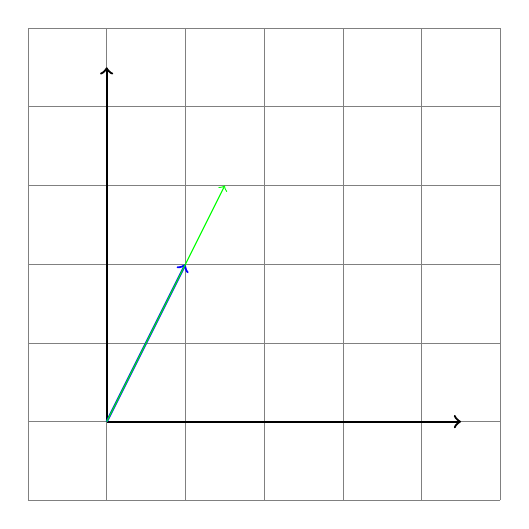
\begin{tikzpicture}
      \draw[step=1cm,gray,very thin] (-1,-1) grid (5,5);
      \draw[thick,->] (0,0) -- (0,4.5);
      \draw[thick,->] (0,0) -- (4.5,0);
      \draw[->,blue,thick] (0,0) -- (1,2);
      \draw[->,green] (0,0) -- (1.5,3);
    \end{tikzpicture}
  \end{center}

  As you can seee, the two vectors overlap, and the only way for a vector to be in their span is to be on the same line. Here are a few examples: 
  \[ \begin{bmatrix}
    -3 \\ -6
  \end{bmatrix} \text{is in the span of } V\]
  \[ \begin{bmatrix}
    0 \\ 0
  \end{bmatrix} \text{is in the span of } V\]
  \[ \begin{bmatrix}
    1 \\ 3
  \end{bmatrix} \text{is not in the span of } V\]
  \end{ex}
  \subsection{Linear Independence}
  Like shown in the previous example, sometimes having 2 vectors in the span doesn't mean that the span will be 2 dimensional. If a vector is a scalar of another one, this means that they are lineary dependent.
  \begin{ex}
    \[
    \begin{bmatrix}
      4 \\ 4
    \end{bmatrix}
    \text{ is linearly dependent to}
    \begin{bmatrix}
      -2 \\ -2
    \end{bmatrix}
    \text{ but is independent from }
    \begin{bmatrix}
      3 \\ 2
    \end{bmatrix}
    \]
  \end{ex}
  \subsection{Spans in 3 dimensions}
  Spans in 3 dimensions work in the exact same way given that only 2 vectors are given in $V$. The span simply creates a 2D place in the 3D space which defines the span. \\
  Adding a 3rd vector that is not within the span of the other 2, will allow for any point in the 3 dimensional space to be within the span. \\
  This 3 dimensional aspect is relatively hard to explain on paper, I recommend you watch \href{https://youtu.be/k7RM-ot2NWY?t=357}{this video} if you don't understand this concept.

  \section{Gaussian Elimination}
  Let's consider a system of 3 simultaneous equations with 3 unknowns:
  \[3x_1+2x_2+x_3 = 39 \]
 \[2x_1+3x_2+x_3 = 34 \]
 \[x_1+2x_2+3x_3 = 26 \]
 Now, to find the value of $x_1, x_2$ and $x_3$, we can use what's called \textbf{Gaussian Elimination}. \\
 Firstly, let's agree on notation. Let $\rho_n$ be the $n_{th}$ equation, so $\rho_1$ would be the first equation ($3x_1 + ... = 39$) and so on. \\
  Firstly, we can replace $\rho_3$ with $\rho_1 - 3\rho_3$ to get rid of $x_1$
  \[
    -4x_2 - 8x_3 = -39
  \]
  Now, we can replace $\rho_2$ with $\rho_1 - \frac{3}{2} \rho_2$ to get rid of $x_1$
  \[
    -\frac{5}{2}x_2 - \frac{1}{2}x_3 = -12
  \]
  The final step is replacing $\rho_3$ with $-\frac{8}{5}\rho_2 + \rho_3$ to get rid of $x_2$
  \[
    -\frac{36}{5}x_3 = -\frac{99}{5}
  \]
  This leaves us with:
  \[ 3x_1+2x_2+x_3=39 \]
  \[-\frac{5}{2}x_2 - \frac{1}{2}x_3 = -12\]
\[
    -\frac{36}{5}x_3 = -\frac{99}{5}
  \]
  The equations can be represented as an \textbf{Augmented matrix} as such:
  \[
    \begin{amatrix}{3}
      3 & 2 & 1 & 39 \\
      0 & \frac{5}{2} & -\frac{1}{2} & -12 \\
      0 & 0 & -36 & -99 \\
    \end{amatrix}
  \]
  This can now be solved by back substitution, but in order to make it easier, we can divide all the rows by the first entry.
  \[\begin{amatrix}{3}
    1 & \frac{2}{3} & \frac{1}{3} & 13 \\
    0 & 1 & \frac{1}{5} & \frac{24}{5} \\
    0 & 0 & 1 & \frac{11}{4} \\
  \end{amatrix} \]
  The form above is called \textbf{echelon form}. In order for an augmented matrix to be in echelon form, it needs to satisfy the following rules:
  \begin{enumerate}
    \item All leading entries in each row are equal to 1
    \item If a column contains a leading entry, then all entries below have to equal 0
    \item In any 2 consecutive non-zero entries, the leading entry in the upper row occurs to the left of the leading entry in the lower row.
  \end{enumerate}
  \end{document}
